\section{Rare-events algorithms}
\label{sec:rare_events_algorithms}

According to Eq.~\eqref{eq:return_time}, the return time of fluctuations $f_d \geq a$ scales like
$r(a)\propto e^{l a}$, meaning that the computational cost required to sample events of amplitude $f_d \geq a$ through brute-force sampling diverges exponentially.
The direct sampling approach used in the previous sections to sample extremes of the drag is therefore not scalable and it would be difficult, if even feasible, to study rarer events or more complex flows.

In this section, we investigate the use of rare-events algorithms in order to sample extreme events for a
computational cost much lower than their return time.
Should this approach be successful, it would pave the way to the simulation of extreme events for flows of
greater complexity than the two-dimensional flow discussed in the previous sections.

We focus on two algorithms, representatives of two popular approaches in rare event simulation.
The first one is the \acl{ams} algorithm \citep{cerou_adaptive_2007} and builds on previous ideas about splitting approaches \citep{KahnHarris1951,glasserman_multilevel_1999}.
In recent years, it has allowed for the computation of rare events in problems involving a large number of degrees of freedom, such as molecular dynamics simulations \citep{aristoff_adaptive_2015,teo_adaptive_2016} or stochastic partial differential equations for the computation of rare trajectories in the Allen-Cahn equations \citep{rolland_computing_2016}. More recently, it has been applied to rare events in stochastic models of wall-turbulence \citep{rolland_extremely_2018} and atmospheric dynamics \citep{bouchet2019rare}.
The second algorithm we consider in this section is the cloning algorithm \citep{giardina_direct_2006}, also known as population dynamics or interacting particles system algorithm.
This approach is very similar to the Diffusion Monte Carlo method used in computational chemistry, and has been introduced and refined in many variants.
Among them the cloning algorithm introduced by Giardina and Peliti \citep{giardina_direct_2006} was successfully applied to chaotic dynamical systems \citep{giardina_simulating_2011,Laffargue_2013}.
More recently it allowed the numerical simulation of extreme heat waves in a simplified model of the atmosphere \citep{ragone_computation_2018}.
This use represents a significant leap in the applicability of rare-event sampling algorithms to complex dynamical systems.
Along the same line, rare-event sampling algorithms are here applied outside of traditional applications by considering fluid-structure interaction in a turbulent flow.

The \ac{ams} is based on the simulation of an ensemble of $N$ independent trajectories $\{\mathbf{x}_n(t)\}_{0\leq t \leq T_a}$ with $n=1 \cdots N$.
Each $\{\mathbf{x}_n(t)\}_{0\leq t \leq T_a}$ refers to a trajectory of duration $T_a$ in the phase space of the
system.
Following the initial simulation of this ensemble, trajectories are iteratively resampled in order to maximise the maximum value of a score function $\xi(\mathbf{x})$ along the trajectories.
The difficulty in applying the \ac{ams} lies in the choice of the score function, which can drastically
influence the effectiveness of the resampling in leading to extreme events \citep{rolland_statistical_2015}.
Mathematical analysis of the \ac{ams} provide proof of existence of an optimal score function, kown as the
committor function. However, with the exception of rare analytical cases, this function is unknown.
See appendix~\ref{app:AMS_on_OU} for a description of the \ac{ams} and its basic mathematical properties.

Similarly to the \ac{ams}, the cloning algorithm simulates an ensemble of trajectories of the system.
However, resampling steps are performed along the simulation of the ensemble.
Trajectories are first evolved independently from $t = 0$ to $t=\tau < T_a$ and then duplicated or pruned
according to the average of an observable $O(\mathbf{x})$ over the interval $[0;\tau]$.
This procedure is then repeated $n-1$ times over the intervals $[\tau, 2\tau], [2\tau, 3\tau]... [(n-1)\tau, n\tau = T_a]$.
Ultimately, the sampled trajectories are distributed according to a probability distribution that is tilted towards large values of the average observable:
\begin{align}
\mathbb{P}_{k}\left(\left\{ \mathbf{X}(t)\right\} _{0\leq t\leq T_{a}}=\left\{ \mathbf{x}(t)\right\} _{0\leq t\leq T_{a}}\right) &\underset{N\rightarrow\infty}{\sim} \frac{e^{k\int_{0}^{T_{a}}O(\mathbf{x}(t))dt}}{Z(k,T_a)}\mathbb{\mathbb{P}}_{0}\left(\left\{ \mathbf{X}(t)\right\} _{0\leq t\leq T_{a}}=\left\{ \mathbf{x}(t)\right\} _{0\leq t\leq T_{a}}\right),
\label{eq:Biased_Path_Approximation_main}
\end{align}
where
$\mathbb{P}_{0}\left(\left\{ \mathbf{X}(t)\right\} _{0\leq t\leq T_{a}} = \left\{ \mathbf{x}(t)\right\} _{0\leq t\leq T_{a}}\right)$ refers formally to the probability of observing the trajectory
$\left\{ \mathbf{x}(t)\right\} _{0\leq t\leq T_{a}}$ according to the unbiased statistics of the model.
See appendix~\ref{app:gktl} for a more detailed description of the cloning algorithm.

Both algorithms are similar in the way that they evolve an ensemble of trajectories, introducing selection
rules to bias the sampling towards extreme events.
In both cases, the output of the algorithm is an ensemble of $N$ trajectories that over-samples the extreme
events of interest.
Note that these trajectories are not statistically independent, however rigorous mathematical results link the statistics sampled by the algorithms to the unbiased statistics of the system, \textit{i.e.} the statistics sampled by a direct sampling approach \citep{DelMoral2013, brehier:hal-01142704}.

Most previous applications of the \ac{ams} and cloning algorithm target stochastic dynamics.
We stress that this is not the case in this work, as the target flow model is fully deterministic.
Because in both algorithms the initial condition of resampled trajectories is taken as the flow state of another, it is therefore required to add a random perturbation to the initial conditions of resampled trajectories, so that they separate from the trajectory they are resampled from.
The amplitude of this perturbation is chosen very low, and it was tested that it does not impact the statistics of the sampled trajectories.
The separation of trajectories under this slight perturbation is guaranteed by the chaoticty of the flow.
For further details about the addition of this perturbation, see appendix~\ref{app:perturb_branching_time}.

\subsection{The \acl{ams} algorithm}
\label{sec:ams}
We applied the \ac{ams} algorithm, described in appendix\ref{app:ams}, to the sampling of extreme fluctuations of the drag applied on the square obstacle immersed in the flow described in section~\ref{sec:test_flow}.
We chose to set the score function as the drag itself, that is $\xi(\mathbf{x}) = f_d(\mathbf{x})$.
Let us stress that we do not expect this choice to be close to the optimal "committor" function.
Because of the complexity of the dynamics, approaching the optimal score function requires intricate insight
into the physics that lead to the extreme events of interest.
Considering further application of the \ac{ams} to complex, three-dimensional flows, such knowledge is out of reach.
It is therefore important to assess the relevance of the application of the algorithm based on a naive choice for the
score function, a choice that is often the only available one.

In addition to the score function, the parameters of the \ac{ams} are the number of trajectories $N$ and the duration of trajectories $T_a$.
As detailed in appendix~\ref{app:ams}, the size of the ensemble $N$ governs the statistical error affecting the estimators based on the sampled set of trajectories.
Furthermore, the number of resamplings required to reach a final ensemble of trajectories of probability of the order of $10^{-\beta}$ can be shown to scale like $\beta N$ \citep{lestang_computing_2018}.
In this work, the choice of $N$ was governed by the available computational resources.
We performed two experiments with $N = 32$ and $N = 256$, having in mind that higher numbers are unlikely to be accessible in the case of more complex or three-dimensional flows.
The duration of the trajectories was set to $T_a$ = $5\tau_c$, a value that is larger than the timescale of extreme drag fluctuations whilst maintaining an affordable computational cost.
As pointed out in appendix~\ref{app:ams}, setting $T_a \gg \tau_c$ does not lead to a better sampling.

\begin{figure}
  \centering
  \subfloat[\label{fig:AMS_drag_trajectories_a} Final ensemble of trajectories sampled by the \ac{ams}]{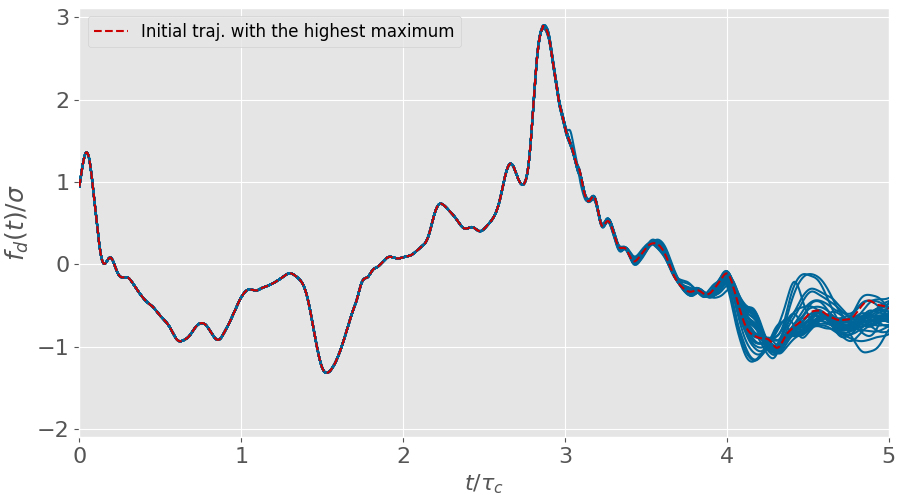
\includegraphics[width=.4\linewidth]{AMS_drag_trajectories/AMS_drag_trajectories.png}}
  \subfloat[Drag maximum for resampled trajectories]{\label{fig:AMS_drag_trajectories_b}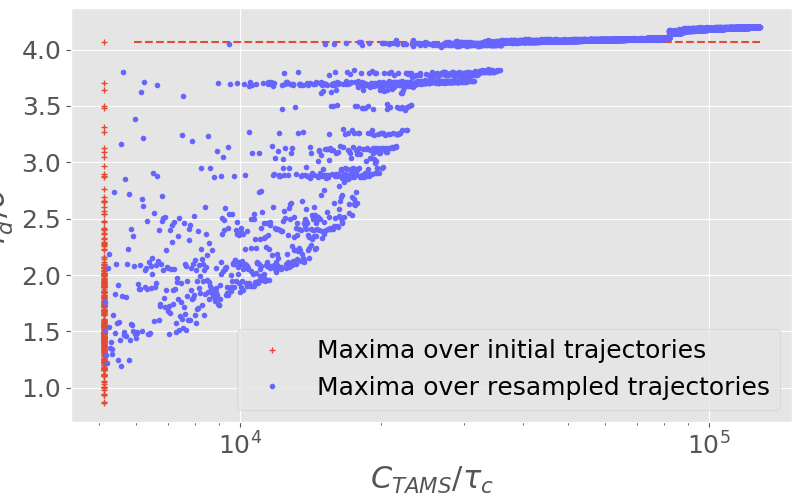
\includegraphics[width=.4\linewidth]{AMS_drag_resampling/AMS_drag_resampling.png}}
  \caption{(a) Ensemble of $N = 32$ trajectories after $181$ \ac{ams} resamplings.
    (b) Maximum of the instantaneous drag throughout the resampled trajectories as a function of the corresponding computational cost $C_{AMS}$, \textit{i.e.} as a function of the resamplings. The maximum over resampled trajectories overlap until saturating at the level of the largest maximum in the initial ensemble.
  }
\end{figure}

Figure~\ref{fig:AMS_drag_trajectories_a} illustrates that the splitting introduced by the \ac{ams} does not enhance the sampling of extremes but rather has catastrophic consequences on the sampling of trajectories.
Indeed, trajectories in the final ensemble overlap over most of their duration and are replicates of the trajectory presenting the largest maximum in the initial ensemble.
This result is confirmed by increasing the number of initial trajectories from $N=32$ to $N=256$, as shown
in figure~\ref{fig:AMS_drag_trajectories_b}.
Recalling section~\ref{sec:instantaneous_drag}, extreme drag fluctuations have a lifetime of $\tau_c$, the timescale over which a vortex is blocked near the base of the obstacle.
After $\tau_c$, the vortex is freed and swept downstream, and further large drag fluctuations can only result from the interaction of the obstacle with the incoming flow, beyond the correlation time of the drag fluctuations.
Moreover, it takes a certain time $\tau_L$ (known as the Lyapunov timescale) before a trajectory resampled by the \ac{ams} separates from its parent under the effect of the initial perturbation.
In our situation, this ``memory effect'' originates from the fact that the score function is of dimension much smaller (here 1) than the dimension of the phase space (very large for this fluid dynamics problem).
%
We observe in Fig.~\ref{fig:AMS_drag_trajectories_a} that this separation timescale is larger than the duration of extreme drag fluctuations $\tau_c$, leading to an overlap of trajectories.

We stress that this phenomenology is independent of the choice of $N$ and $T_a$.
Increasing the size of the initial ensemble can only increase the amplitude of the the global maximum attained initially, but does not solve the issue of overlapping trajectories.
Increasing $T_a$ allows further time for resampled trajectories to develop rare fluctuations, however after a duration $\Delta T \geq \tau_L > \tau_c$, and therefore decorrelated from the resampling.

Our results indicate that the \ac{ams} does not work with this simple choice of score function.
Better results may be obtained by using a different score function, but at this stage we do not know how to build such a score function for this specific problem.

\subsection{The \ac{gktl} algorithm}
\label{sec:gktl}
We applied the cloning algorithm described, in appendix\ref{app:gktl}, to the two-dimensional flow described in section~\ref{sec:test_flow}.
Unlike the case of the \ac{ams} in section~\ref{sec:ams}, the algorithm is here used to sampled trajectories that exhibit extremes values of
the \emph{average} drag.

The cloning algorithm depends on three parameters: the cloning strength $k$, the number of trajectories $N$ and the resampling period $\tau$.
The cloning strength is the multiplicative factor appearing the the bias term of equation~\eqref{eq:Biased_Path_Approximation_main}.
The higher $k$, the larger the typical average drag for the trajectories in the ensemble sampled by the algorithm.
There is however no general relation between this typical value and the value of $k$, and this value must be set empirically.
Similarly to the \ac{ams}, $N$ governs the error affecting estimates of probabilities and estimators based on the biased ensemble.
In the cloning algorithm, the population of trajectories is periodically resampled as the trajectories are simulated from $t=0$ to
$t=T_a$.
The cloning period determines how often this resampling step is performed.
For deterministic dynamics, a common rule of thumb is to chose $\tau \approx \tau_c$ \citep{giardina_direct_2006}.
For further details about the cloning algorithm, see appendix~\ref{app:gktl}.

In practice, we started by fixing the computational cost associated with a single run of the cloning algorithm, \textit{i.e.} by fixing $N \times T_a$.
Consistently with section~\ref{sec:time_avg}, we aim at sampling trajectories with a duration $T = 10\tau_c$.
Consequently, we fixed $T_a = 15\tau_c$ to allow for an initial transient regime of the cloning algorithm.
Then, we chose $N = 1024$ to obtain a computational cost of order $\mathcal{O}(10^4 \tau_c)$, \textit{i.e.} roughly one hundredth of the computational cost associated with the direct numerical simulation used for direct sampling in section~\ref{sec:direct_sampling}.
Finally, we set $\tau = \tau_c / 2$.

\begin{figure}
  \centering
  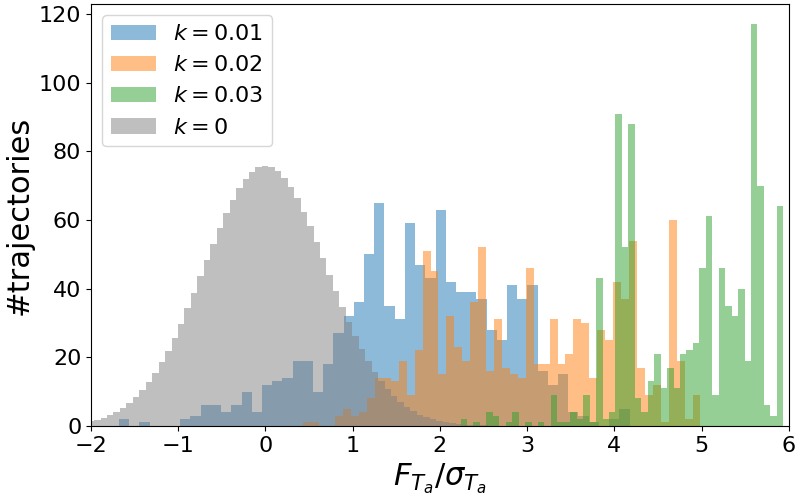
\includegraphics[width=.7\linewidth]{IS_GKTL/IS_GKTL_2}
  \caption{Histogram of the values of the time-averaged drag $F_{T_a}$, with $T_a = 10\tau_c$, in the ensemble sampled by the cloning algorithm, for three values of the cloning strength $k$. In each case, the algorithm was applied with $N=1024$, $\tau = \tau_c / 2$. The grey histogram represents the average histogram obtained through a direct sampling, \textit{i.e.} with $k=0$. It was computed using a Gaussian approximation for the \ac{pdf} of the time-averaged drag.}
  \label{fig:IS_GKTL}
\end{figure}
Figure~\ref{fig:IS_GKTL} shows the histogram of the values of the average drag $F_{T_a} = \frac{1}{T_a}\int_{0}^{T_a}f_d(t)\mathrm{d}t$ for three ensemble of trajectories sampled with three different values of the cloning strength $k$.
It illustrates that the algorithm effectively samples preferentially trajectories with a higher value of the average.
The higher $k$, the stronger the bias.
The grey histogram represents the average histogram that would be obtained using a direct approach -- \textit{i.e.} with $k=0$ -- for the same computational cost.
We computed this histogram by approximating the \ac{pdf} of the drag averaged over $10\tau_c$ as a Gaussian \ac{pdf} (see figure~\ref{fig:PDF_AVG}).
Figure~\ref{fig:IS_GKTL} also illustrates that the sampling by the algorithm is very concentrated on some fluctuations values, and that this effect increases as $k$ increases.
This results from the overlap of trajectories as a consequence of the cloning and pruning.
Indeed, if a trajectory is cloned at step $i$, then the trajectory ${\mathbf{x}(t)}$ over the interval $[0;i\tau]$ will be the same for all the clones.
For a fixed ensemble size $N$, the overlap of trajectories increases as $k$ increases as fewer
trajectories are cloned into a higher number of duplicates.
\textbf{How do we quantify this effect? It is probably application-dependant. What are the strategies to mitigate it?}

Figure~\ref{fig:timeseries_extrms_AVG_GKTL} displays the drag timeseries for several trajectories within the ensemble sampled by the cloning algorithm.
It illustrates that the cloning algorithm samples trajectories that exhibit successive positive fluctuations, resulting in a very large value of the average drag.
Note that during the post-processing of the sampled trajectories, trajectories overlapping over more than half of their duration ($5 \tau_c$) have been considered duplicates, and treated as effectively the same trajectory.
This procedure resulted in an ensemble of ?? "distinct" trajectories (out of the original $N = 1024$).

\begin{figure}
  \centering
  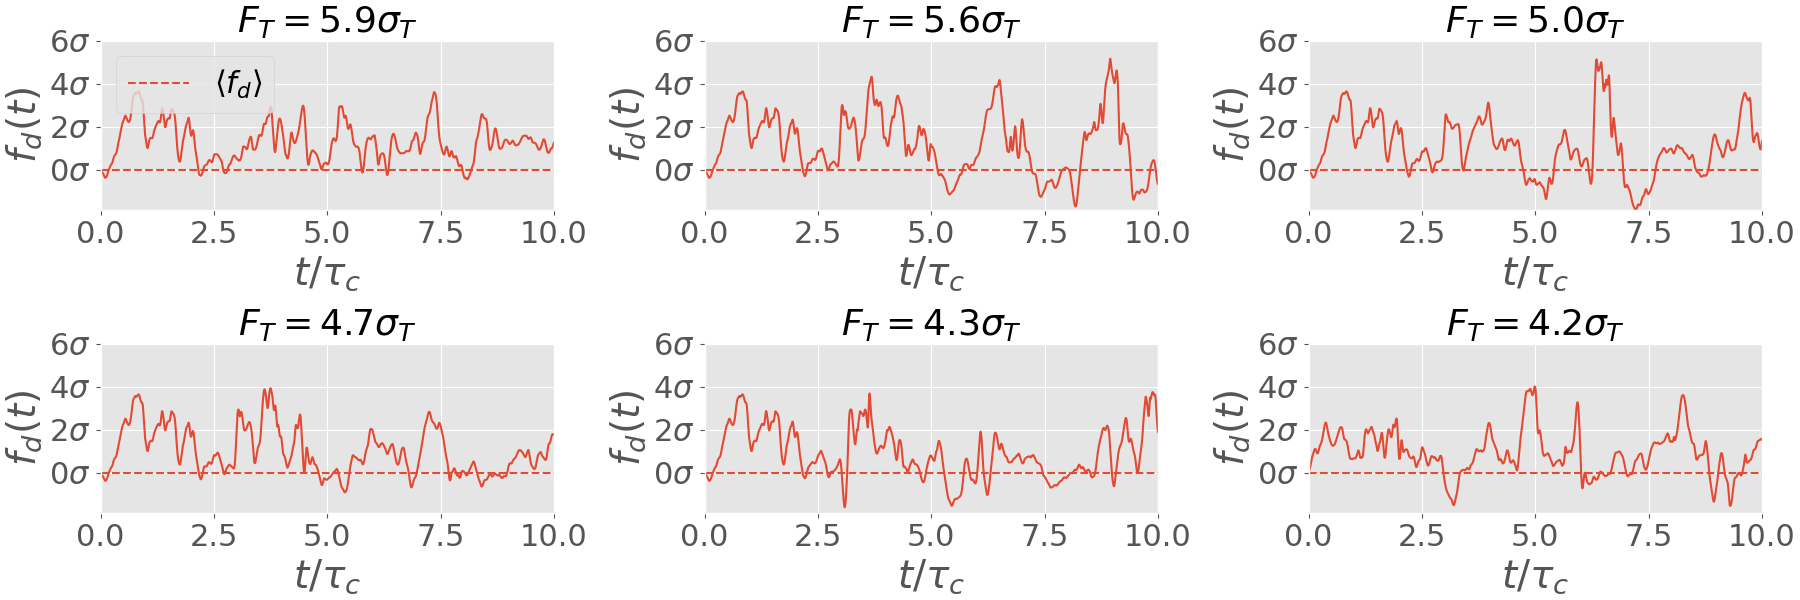
\includegraphics[width=\linewidth]{timeseries_extrms_AVG_GKTL/timeseries_extrms_AVG_GKTL}
  \caption{Drag timeseries corresponding to the 6 highest fluctuations of the average drag in the ensemble sampled by the cloning algorithm. The cloning algorithm was applied with $N = 1024$, $\tau = \tau_c / 2$ and $k = 0.03$. }
  \label{fig:timeseries_extrms_AVG_GKTL}
\end{figure}

In addition, figure~\ref{fig:illustr_extrms_vorticity_GKTL} displays the vorticity field at the time of maximum drag over a subset of trajectories
sampled by the cloning algorithm.
It shows that the sampled events are consistent with the picture of strong vorticity levels being concentrated in the vicinity of the base of the obstacle, as pointed out in section~\ref{sec:instantaneous_drag}.
Moreover, we stress that the computational cost for the sampling of the events shown in figures~\ref{fig:timeseries_extrms_AVG_GKTL} and~\ref{fig:illustr_extrms_vorticity_GKTL} is roughly a hundredth of computational cost of the direct sampling required to sample events shown in figures~\ref{fig:extreme_avg} and~\ref{fig:top_4_events_vorticity}.

\begin{figure}
  \centering
  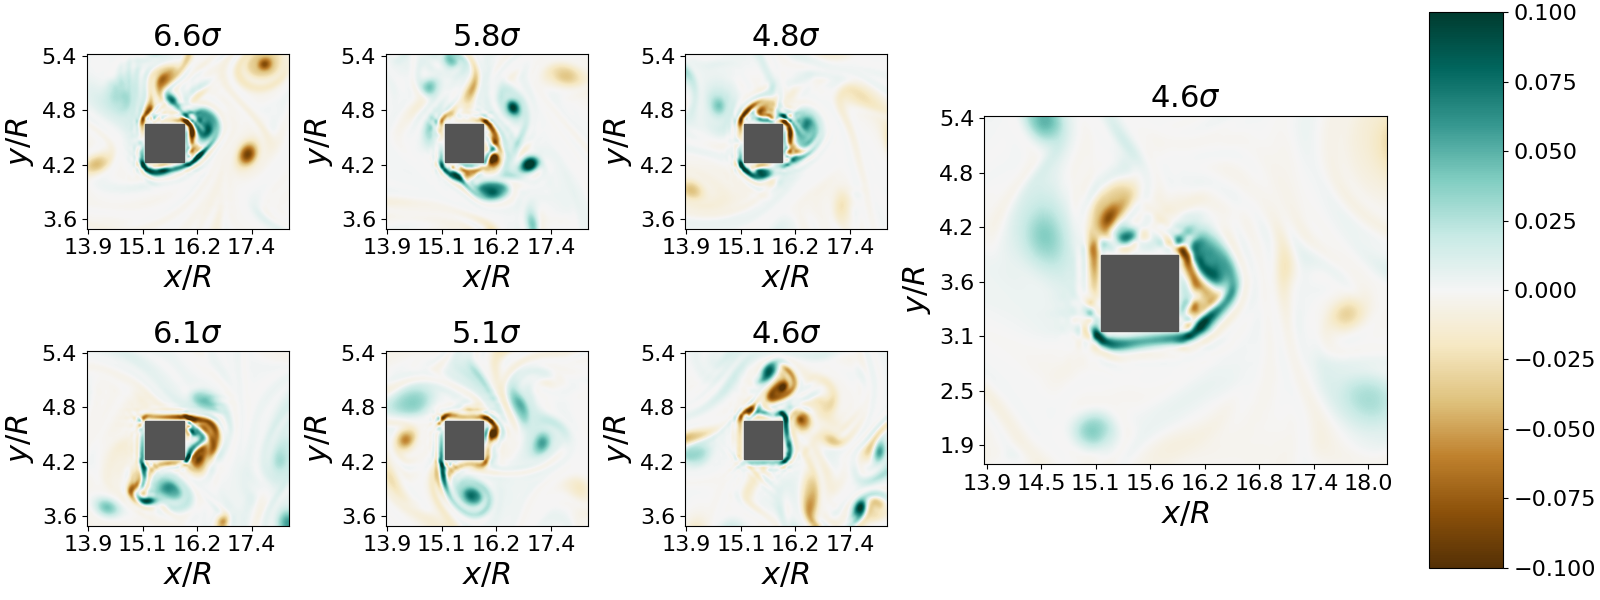
\includegraphics[width=\linewidth]{illustr_extrms_vorticity_GKTL/illustr_extrms_vorticity_GKTL}
  \caption{Vorticity field corresponding the maximum of the drag $f_d$ over trajectories sampled by the cloning algorithm.}
  \label{fig:illustr_extrms_vorticity_GKTL}
\end{figure}

An important remaining question is whether or not the sampled ensemble of trajectories are representative of the full range of dynamics that can lead to extreme values of the average drag.
Indeed, it was observed in section~\ref{sec:time_avg} that large values of the average drag over $10\tau_c$ can result from a variety of different
dynamics, including the succession of independent positive fluctuations, but also the occurrence of fewer and larger fluctuations separated by periods of typical drag.
In particular, it is not clear from the results of the present work whether or not the cloning algorithm is suited to sample trajectories of the latter form.
A possible continuation of this study is to go beyond the qualitative description of the events sampled by the cloning algorithm, a task that is left to future work.

\subsubsection{Computation of return times}
\label{sec:return_times}

Beyond dynamical aspects, the cloning algorithm provides ensemble of trajectories over which statistics of rare events can be computed by inverting Eq.~\eqref{eq:Biased_Path_Approximation_main}.
In this section, we show that the biased sampling performed by the cloning algorithm allows for the computation of return times for events otherwise out-of-reach from a direct sampling approach.

Each trajectory $j$ in the biased ensemble results in a timeseries of the time-averaged drag:
\begin{equation}
\label{eq:time_averaged}
F_T^{(j)}(t) = \int_{t-T}^{t}f_d^{(j)}(\tau)d\tau, \quad t\in [T,T_a]  ,
\end{equation}
and the return time of a fluctuation $F_T \geq a$ is given by~\citep{lestang_computing_2018}
\begin{equation}
r(a) = - \frac{T_a - T}{\ln (1-\mathbb{P}(F_T \geq a))}.
\end{equation}


The probability $\mathbb{P}(F_T \geq a)$ can be estimated from the biased ensemble by inverting Eq.~\eqref{eq:Biased_Path_Approximation_main}
\begin{equation}
  \mathbb{P}(f_d \geq a) \approx \frac{1}{N}\sum_{j=1}^{N}e^{T_a \lambda(k)}e^{kT_aF_T^{(j)}}s_j(a),
\end{equation}
with $s_j(a) = 1$ if $\max_{T\leq t \leq T_a}[F_T^{(j)}] \geq a$ and $s_j(a) = 0$ otherwise. This amounts to taking the sum of the weights of the timeseries which maximum is larger than $a$.

Fig.~\ref{fig:return_times_gktl} displays the return times for extreme fluctuations of the time-averaged drag acting on the square obstacle.
Two independent estimates are shown, obtained using different values of the cloning strength $k$.
Note that both estimates have been computed with the same computational cost $T_{tot}=N\times T_a$.
In addition, figure~\ref{fig:return_times_gktl} shows an estimate computed through direct sampling with the same computational cost, \textit{i.e.} using a timeseries of duration $T_{tot}$.
Whilst a direct approach cannot access events with a return time greater than $T_{tot}$, the cloning algorithm allows for the computation of statistics of drag fluctuations having a return time several orders of magnitude above $T_{tot}$.
This result shows that the biased ensemble sampled by cloning algorithm enables the estimation of return times for average drag fluctuations that would be out-of-reach from a direct sampling.
Alternatively, for a fixed target return time, the use of the cloning algorithm can reduce the computational cost of the estimation by several orders of magnitude.
This is obviously a major advantage of this rare-event sampling algorithm.

More generally, the successful computation of return times indicates that, despite the complex dynamics and the overlapping trajectories, the biased ensemble generated by the cloning algorithm may be used to compute statistical estimators in a very efficient manner.
We note, however, that some estimators may be more affected by the quality of the sampling than others.

\begin{figure}
  \centering
  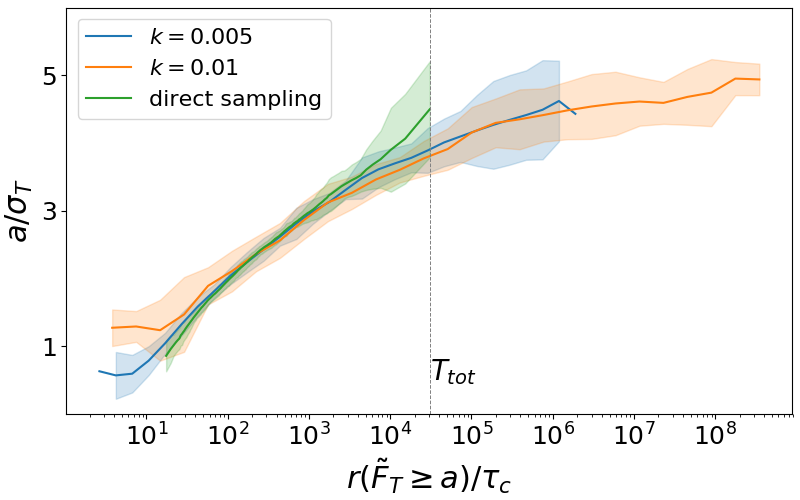
\includegraphics[width=.7\linewidth]{return_times_GKTL/return_times_GKTL}
  \caption{\label{fig:return_times_gktl} Return times for the time-averaged drag acting on the square obstacle. $\tilde{F}_T$ denotes the time-averaged drag with zero mean. The blue and red lines are obtained from the biased ensemble of trajectories generated by the \ac{gktl} algorithm with $N=1024$ and $T_a=30\tau_c$. The green line is the return times obtained from a single timeseries of duration equal to the computational cost of both \ac{gktl} experiments. Uncertainty ranges for the \ac{gktl} estimates are computed as the standard deviation over a set of 10 independent experiments. Uncertainty ranges for the direct estimation are computed as the standard deviation over a ensemble of direct estimates resulting from 60 independent timeseries.}
\end{figure}


%%% Local Variables:
%%% mode: latex
%%% TeX-master: "draft_p2_jfm"
%%% End:
